\documentclass[a4paper,12pt]{book} %размер бумаги устанавливаем А4, шрифт 12пунктов
\usepackage[T2A]{fontenc}
\usepackage[utf8]{inputenc}%включаем свою кодировку: koi8-r или utf8 в UNIX, cp1251 в Windows
\usepackage[english,russian]{babel}%используем русский и английский языки с переносами
\usepackage{amssymb,amsfonts,amsmath,mathtext,cite,enumerate,float,alltt} %подключаем нужные пакеты расширений
\usepackage{longtable}
\usepackage[dvips]{graphicx} %хотим вставлять в диплом рисунки?
\usepackage{dirtree}
\graphicspath{{images/}}%путь к рисункам

\makeatletter
\renewcommand{\@biblabel}[1]{#1.} % Заменяем библиографию с квадратных скобок на точку:
\makeatother

\usepackage{geometry} % Меняем поля страницы
\geometry{left=2cm}% левое поле
\geometry{right=1.5cm}% правое поле
\geometry{top=1cm}% верхнее поле
\geometry{bottom=2cm}% нижнее поле

\renewcommand{\theenumi}{\arabic{enumi}}% Меняем везде перечисления на цифра.цифра
\renewcommand{\labelenumi}{\arabic{enumi}}% Меняем везде перечисления на цифра.цифра
\renewcommand{\theenumii}{\arabic{enumii}}% Меняем везде перечисления на цифра.цифра
\renewcommand{\labelenumii}{\arabic{enumi}.\arabic{enumii}.}% Меняем везде перечисления на цифра.цифра
\renewcommand{\theenumiii}{\arabic{enumiii}}% Меняем везде перечисления на цифра.цифра
\renewcommand{\labelenumiii}{\arabic{enumi}.\arabic{enumii}.\arabic{enumiii}.}% Меняем везде перечисления на цифра.цифра

\begin{document}

\bibliography{lectures}

\begin{titlepage}
\title{\Huge \textbf{UNIX и Linux. \\ Архитектура, Идеология, \\ Администрирование.}}
\author{Авторы: Николай Замотаев, Петрова Ольга, Никонов Данил}
\maketitle

\end{titlepage}
% это титульный лист
\tableofcontents % это оглавление, которое генерируется автоматически

\chapter {История unix}
\section {Рождение}
UNIX родился в 1969 году, как учебный проект, на малоиспользуемой PDP-8 ???? что стояла в углу.
Первоначально UNIX был написан на ассемблере, но уже в 1971 году был переписан на C, с целью облегчения понимания и портируемости. В результате стало возможным портирование UNIX на другие системы с минимальными модификациями (только ассемблерные вставки, без изменения C-кода).
\section {Развитие}
\subsection {Коммерческий UNIX}
UNIX стал популярен в результате одного исторического решения: AT\&T стала раздавать UNIX университетам, вместе с исходным кодом (для возможности модификации под свои нужды). Это, а так же то, что UNIX в тот момент был достаточно прост (порядка 10000 строк кода), привело к тому, что учебные курсы стали ориентироваться на UNIX, и изучать его устройство. Как следствие это привело к распространению популярности UNIX-а за пределы университетской среды вместе с выпускниками.
\subsection {Свободные альтернативы}
Следующей исторической вехой стоит назвать создание Ричардом Столлманом FSF (Free Software Foundation) в 1984??? году. 

В 1991 году Линус Торвальдс ???
%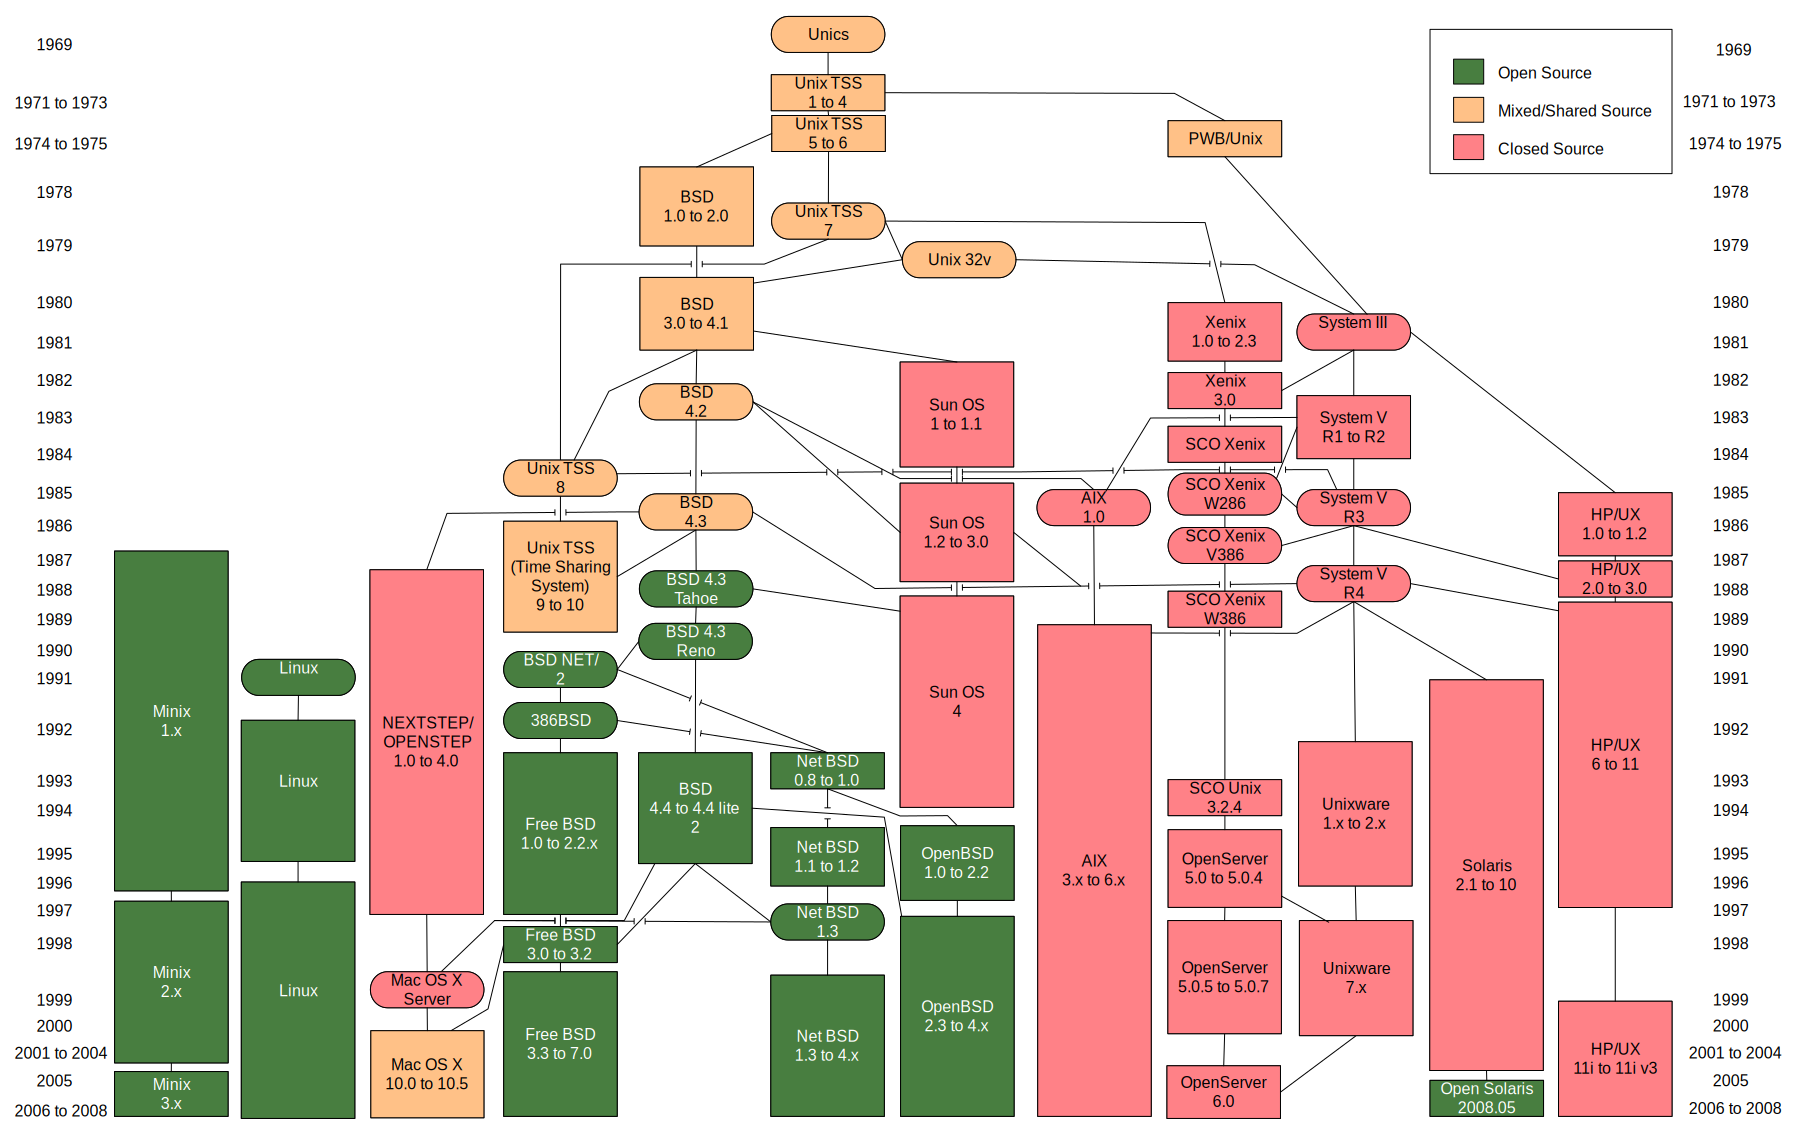
\includegraphics{unix_history}
\section {Стандарты}
\subsection {Single UNIX Specification}
Single UNIX Specification это общее название стандартов, которым должна соответствовать операционная система, чтобы называться «Unix». SUS разрабатывается и поддерживается Austin Group на основе предыдущих разработок IEEE и The Open Group.
\subsection {Степени совместимости и версии стандарта}
Существуют несколько степеней совместимости, нумерующихся по году:
\begin{enumerate}
\item UNIX 93
\item UNIX 95
\item UNIX 98 (удовлетворяет SUS версии 2 ( частичная совместимость )
\item UNIX 03 (удовлетворяет SUS версии 3 ( полная совместимость )
\end{enumerate}
\subsection{Зарегистрированные UNIX-подобные системы}

AIX
    AIX 5L V5.2 с обновлениями, AIX 5L V5.3 и AIX 6.1 совместимы с UNIX 03. AIX 5L V5.2 совместима с UNIX 98.

HP-UX
    HP-UX 11i V3 Release B.11.31 совместима с UNIX 03. Предыдущие версии совместимы с UNIX 95.

IRIX
    IRIX 6.5.28 совместима с UNIX 95.

Mac OS X
    Mac OS X 10.5 «Leopard» и Mac OS X Server 10.5 «Leopard Server» на процессорах Intel совместимы с UNIX 03.

SCO
    UnixWare 7.1.3 совместима с UNIX 95. SCO OpenServer 5 совместима с UNIX 93.

Solaris
    Solaris 10 совместима с UNIX 03 на системах SPARC, 32-/64-битных системах x86 и SPARC64 (Fujitsu PRIMEPOWER). Solaris 8 и 9 совместимы с UNIX 98 на тех же платформах за исключением 64-битных x86. Solaris 2.5.1 была совместима с UNIX 95 на платформе PReP PowerPC в 1996, но продукт был отменён до начала массовых продаж.

Tru64
    Tru64 UNIX V5.1A и далее совместимы с UNIX 98.

z/OS
    IBM z/OS до 1.9 совместима с UNIX 95.

Поставщики Unix-подобных систем, таких как BSD, OpenSolaris и Linux обычно не сертифицируют свои дистрибутивы из-за высокой цены на сертификацию и высокой скорости изменений в этих системах. Схожий стандарт LSB, используемый некоторыми ОС GNU/Linux, опирается на некоторые части SUS.
\section{POSIX}
POSIX
POSIX (англ. Portable Operating System Interface for Unix — Переносимый интерфейс операционных систем Unix) — набор стандартов, описывающих интерфейсы между операционной системой и прикладной программой. Стандарт создан для обеспечения совместимости различных UNIX-подобных операционных систем и переносимости прикладных программ на уровне исходного кода, но может быть использован и для не-Unix систем. Серия стандартов POSIX была разработана комитетом 1003 IEEE. Международная организация по стандартизации (ISO) совместно c Международной электротехнической комиссией (IEC) приняли данный стандарт (POSIX) под названием ISO/IEC 9945.

Название «POSIX» было предложено Ричардом Столлманом. Введение в POSIX.1 гласит: «Ожидается произношение „поз-икс“ как „позитив“, а не „по-сикс“. Произношение опубликовано в целях обнародования стандартного способа ссылки на стандартный интерфейс операционной системы». «POSIX» является зарегистрированным товарным знаком IEEE.[1]

    * 1 Задачи
    * 2 Состав
    * 3 Версии
    * 4 POSIX-совместимые ОС
          o 4.1 Полностью POSIX-совместимые
          o 4.2 По большей части POSIX-совместимые
                + 4.2.1 POSIX для Windows
    * 5 Примечания
    * 6 Литература
    * 7 См. также
    * 8 Ссылки
\subsection{Задачи}
\begin{enumerate}
\item содействие облегчению переноса кода прикладных программ на иные платформы
\item определению и унификация интерфейсов заранее при проектировании, а не в процессе их реализации
\item сохранить по возможности и учитывать все главные, созданные ранее и используемые прикладные программы; ?????
\item определение необходимого минимума интерфейсов прикладных программ, для ускорения создания, одобрения и утверждения документов
\item развитие стандартов в направлении обеспечения коммуникационных сетей, распределенной обработки данных и защиты информации
\item рекомендовать ограничивать использование бинарного (объектного) кода для приложений в простых системах. ?????
\end{enumerate}
\subsection{Состав}
Стандарт состоит из четырёх основных разделов:

\begin{itemize}
\item Основные определения (Base definitions) — список основных определений и соглашений, используемых в спецификациях, и список заголовочных файлов языка Си, которые должны быть предоставлены соответствующей стандарту системой.
\item Оболочка и утилиты (Shell and utilities) — описание утилит и командной оболочки sh, стандарты регулярных выражений.
\item Системные интерфейсы (System interfaces) — список системных вызовов языка Си.
\item Обоснование (Rationale) — объяснение принципов, используемых в стандарте.
\end{itemize}
Помимо основного стандарта (POSIX.1), cуществуют расширения: POSIX.1b и POSIX.1c. Первое из них относится к расширениям реального времени, второе к threads или потоковому выполнению.

POSIX-совместимые ОС

В зависимости от степени совместимости со стандартами, ОС могут быть полностью или частично совместимы с POSIX. Сертифицированные продукты могут быть найдены на сайте IEEE.
Полностью POSIX-совместимые

Полностью соответствующие одной из версий стандарта POSIX: Android OS, A/UX, BSD/OS, HP-UX, IBM AIX, INTEGRITY, IRIX, LynxOS, Mac OS X, Apple iOS, Minix, MPE/iX, OpenSolaris, OpenVMS, QNX, RTEMS, Solaris, UnixWare, velOSity, VxWorks

По большей части POSIX-совместимые

Официально не сертифицированные как POSIX-совместимые, но соответствующие по большей части.
\begin{itemize}
 \item BeOS
 \item FreeBSD
 \item Linux (большинство дистрибутивов — см. LSB)
 \item NetBSD
 \item Nucleus RTOS
 \item OpenBSD
 \item RTEMS
 \item Sanos
 \item SkyOS
 \item Syllable
 \item VSTa
 \item Symbian OS (при помощи PIPS)
\end{itemize}
\subsection{POSIX для Windows}
\begin{itemize}
\item Cygwin — обеспечивает частичное соответствие POSIX для некоторых продуктов Microsoft Windows.
\item Microsoft POSIX subsystem, необязательная подсистема Windows.
\item Microsoft Windows Services for UNIX — обеспечивает полное соответствие POSIX для некоторых продуктов Microsoft Windows. Операционные системы на базе Windows NT до Windows 2000 имели POSIX уровень встроенный в ОС, и UNIX Services for Windows предоставляло UNIX-подобное окружение. Для Windows XP, Windows Services for UNIX должны быть установлены для POSIX совместимости. UNIX подсистема встроена в Enterprise и Ultimate редакции Windows Vista, и не могут быть добавлены в другие редакции.
\item UWIN от ATnT Research обеспечивает POSIX поверх Win32 API.
\end{itemize}
\section{LSB}
Linux Standard Base, LSB — совместный проект нескольких дистрибутивов Linux при организации Linux Foundation, целью которого является стандартизация внутренней структуры операционных систем, основанных на Linux. LSB опирается на существующие спецификации, такие как POSIX, Single UNIX Specification, и другие открытые стандарты, при этом расширяя и дополняя их.

    Цель LSB — разработать и продвигать набор стандартов, который увеличит совместимость различных дистрибутивов Linux и даст возможность запускать приложения на любой совместимой системе. Кроме того, LSB поможет скоординировать усилия в привлечении разработчиков к написанию и портированию приложений под Linux.

Чтобы сертифицировать программный продукт на совместимость со стандартом LSB, нужно пройти сертификационную процедуру, которая проводится The Open Group сотрудничающей с Free Standards Group.

LSB специфицирует: стандартные библиотеки, несколько команд и утилит в дополнение к стандарту POSIX, структуру иерархии файловой системы, уровни запуска и различные расширения системы X Window System.

    * 2 История версий
    * 3 Стандарт ISO
    * 4 Примечания
    * 5 См. также
    * 6 Ссылки

Стандарт LSB критикуют за то, что он не принимает предложения проектов, в особенности Debian, находящихся за пределами круга его членов.

К примеру, LSB предписывает поставлять программные пакеты (packages) в формате RPM, который был разработан гораздо позже формата deb, однако разработчики Debian не собираются менять свой формат, так как считают его лучше RPM.

Стандарт не навязывает операционным системам, какой формат им использовать для собственных пакетов. Он лишь говорит, какой формат совместимые системы должны поддерживать для установки приложений сторонних разработчиков.

Так как в Debian присутствует опциональная поддержка LSB (версии 1.1 в woody, 2.0 в sarge, а позднее 3.1 в etch и 3.2 в lenny), проблема исчезает при более близком рассмотрении (то есть пользователь всего лишь должен использовать утилиту alien для преобразования и установки сторонних пакетов). Таким образом, на практике Debian совместим с LSB.

Известный в сообществе открытого программного обеспечения программист Ульрих Дреппер критиковал LSB за плохое качество тестирования, которое может привести к несовместимости между сертифицированными дистрибутивами. ??? (Ага, щаз, а у самого glibc собирается только с bash и никак иначе).

Он также указывал на недостаток тестов для приложений, отмечая, что тестирование только дистрибутивов никогда не решит проблем приложений, полагающихся на особенности конкретных реализаций.

Первая версия LSB была выпущена в июне 2001. Текущая версия, 4.0 выпущена в 2008 году.

LSB зарегистрирован в качестве официального стандарта ISO. (ISO/IEC 23360).
\section {FHS}
FHS — сокращение от Filesystem Hierarchy Standard, что в переводе c английского означает «Стандарт иерархии файловой системы». Этот стандарт принят для унификации местонахождения файлов и директорий с общим назначением в файловой системе ОС UNIX. На данный момент большинство UNIX-подобных систем в той или иной степени следует этим правилам. Например, обычная база данных о пользователях всегда хранится в файле /etc/passwd.

Текущая версия стандарта — 2.3, анонсирована 29 января 2004 г.

Для получения справки об используемой в ОС системе каталогов иногда существует команда hier (man hier).
Содержание

    * 1 Основные сведения
    * 2 Структура директорий
    * 3 Заметки
    * 4 См. также
    * 5 Ссылки

Основные сведения

Процесс разработки стандарта иерархии файловой системы начался в августе 1993 года с попыток упорядочить структуру директорий и файлов в операционной системе GNU/Linux. 14 февраля 1994 года был выпущен FSSTND (Filesystem Standard), стандарт файловой системы, специфичной для GNU/Linux. Последующие версии были выпущены 9 октября 1994 года и 28 марта 1995 года.

В начале 1996 года сообщество разработчиков BSD присоединилось к разработке новой версии FSSTND с целью разработать стандарт, пригодный для всех Unix-подобных операционных систем. Имя стандарта при этом было изменено на Filesystem Hierarchy Standard (FHS).

FHS поддерживается Free Standards Group — некоммерческой организацией, в составе которой находятся крупные разработчики программного и аппаратного обеспечения, такие как HP, Red Hat, IBM и Dell. Однако основная часть разработчиков дистрибутивов, включая и тех, кто входит в состав Free Standards Group, не следуют стандарту на 100 \%. В частности, пути, специально созданные группой, такие как /srv/, практически нигде не используются. Некоторые Linux-системы отвергают FHS и следуют своему собственному стандарту, как, например, GoboLinux.
Так как FHS начиналась как инициатива Linux-сообщества, другие UNIX и UNIX-подобные операционные системы полностью игнорируют её в пользу своих собственных систем, которые иногда распространены довольно широко. Например, Mac OS X использует такие имена, как /Library/, /Applications/ и /Users/ вместе с традиционными именами UNIX-иерархии.
\subsection{Структура директорий}

В FHS все файлы и директории находятся внутри корневой директории, даже если они расположены на различных физических носителях. Однако некоторые из директорий могут присутствовать только в случае, если установлено определённое программное обеспечение, такое как, например, X Window System. Большая часть этих директорий существует во всех UNIX-подобных операционных системах и используется похожим образом.
\dirtree{%
.1 /.
.2 bin.
.2 boot.
.2 dev.
.2 etc.
.3 opt.
.3 X11.
.3 sgml.
.3 xml.
.2 home.
.2 lib.
.2 media.
.2 mnt.
.2 opt.
.2 proc.
.2 root.
.2 sbin.
.2 srv.
.2 tmp.
.2 usr.
.3 bin.
.3 include.
.3 lib.
.3 sbin.
.3 share.
.3 src.
.3 X11R6.
.3 local.
.4 bin.
.4 include.
.4 lib.
.4 sbin.
.4 share.
.2 var.
.3 lib.
.3 lock.
.3 log.
.3 mail.
.3 run.
.3 spool.
.4 mail.
.3 www.
.3 tmp.
}
\begin{table}
\caption{Иерархия каталогов в FHS}
\label{tabular:fhs}
\begin{center}
\begin{tabular}{|l|p{0.7\linewidth}|}
\hline
Директория & 	Описание \\
/  &	Корневая директория, содержащая всю файловую иерархию. \\
/bin/ & 	Основные утилиты, необходимые как в однопользовательском режиме, так и при обычной работе всем пользователям (например: cat, ls, cp). \\
/boot/ & 	Загрузочные файлы (в том числе файлы загрузчика, ядро, initrd, System.map). Часто выносится на отдельный раздел. \\
/dev/ &	Основные файлы устройств (например, /dev/null, /dev/zero). \\
/etc/ &	Общесистемные конфигурационные файлы (имя происходит от et cetera). \\
/etc/opt/ & Файлы конфигурации для /opt/. \\
/etc/X11/ & Файлы конфигурации X Window System версии 11. \\
/etc/sgml/ & Конфигурационные файлы SGML. \\
/etc/xml/ & Конфигурационные файлы XML. \\
/home/ & 	Содержит домашние директории пользователей, которые в свою очередь содержат персональные настройки и данные пользователя. Часто размещается на отдельном разделе. \\
/lib/ &	Основные библиотеки, необходимые для работы программ из /bin/ и /sbin/. \\
/media/ & 	Точки монтирования для сменных носителей, таких как CD-ROM, DVD-ROM (впервые описано в FHS-2.3). \\
/mnt/ & 	Содержит временно монтируемые файловые системы. \\
/opt/ & 	Дополнительное программное обеспечение. \\
/proc/ & 	Виртуальная файловая система, представляющая состояние ядра операционной системы и запущенных процессов в виде файлов. \\
/root/ & 	Домашняя директория пользователя root. \\
/sbin/ & 	Основные системные программы для администрирования и настройки системы, например, init, iptables, ifconfig. \\
/srv/ &	Данные, специфичные для окружения системы. \\
/tmp/ &	Временные файлы (см. также /var/tmp). \\
/usr/ &	Вторичная иерархия для данных пользователя; содержит большинство пользовательских приложений и утилит, используемых в многопользовательском режиме. Может быть смонтирована по сети только для чтения и быть общей для нескольких машин. \\
/usr/bin/ & Дополнительные программы для всех пользователей, не являющиеся необходимыми в однопользовательском режиме. \\
/usr/include/ & Стандартные заголовочные файлы. \\
/usr/lib/ & Библиотеки для программ, находящихся в /usr/bin/ и /usr/sbin/. \\
/usr/sbin/ & Дополнительные системные программы (такие как демоны различных сетевых сервисов). \\
/usr/share/ & Архитектурно-независимые общие данные. \\
/usr/src/ & Исходные коды (например, здесь располагаются исходные коды ядра). \\
/usr/X11R6/ & X Window System, версии 11, релиз 6. \\
/usr/local/ &	Третичная иерархия для данных, специфичных для данного хоста. Обычно содержит такие поддиректории, как bin/, lib/, share/. \footnote{Где эта чёртова иерархия?} \\
/var/ & 	Изменяемые файлы, такие как файлы регистрации (log-файлы), временные почтовые файлы, файлы спулеров. \\
/var/lib/ &	Информация о состоянии. Постоянные данные, изменяемые программами в процессе работы (например, базы данных, метаданные пакетного менеджера и др.). \\
/var/lock/ &	Лок-файлы, указывающие на занятость некоторого ресурса. \\
/var/log/ &	Различные файлы регистрации (log-файлы). \\
/var/mail/ &	Почтовые ящики пользователей. \\
/var/run/ &	Информация о запущенных программах (в основном, о демонах). \\
/var/spool/ &	Задачи, ожидающие обработки (например, очереди печати, непрочитанные или неотправленные письма). \\
/var/spool/mail/ &	Местоположение пользовательских почтовых ящиков (устаревшее). \\
/var/www/ &	Файлы веб-сайтов (например, иерархия файлов виртуальных хостов). \\
/var/tmp/ &	Временные файлы, которые должны быть сохранены между перезагрузками \\
\hline
\end{tabular}
\end{center}
\end{table}

 %история и идеология unix
\chapter {Идеология unix}
\section {Компоненты}
\subsection{ядро ОС}
\subsection{средства инициализации системы}
\subsection{системные утилиты, обеспечивающие исполнение ядром его функций}
\subsection{средства "боевого обеспечения" - минимальный набор пользовательских утилит}
\subsection{средства "тылового обеспечения" - системные библиотеки}
\subsection{командная оболочка}
\subsection{система документации}
\section {Основные принципы}
\subsection{всё есть поток байтов}
\subsection{лень читать вывод программы - дай это другой программе или конвеер}
\subsection{модульность - программа должна делать одно дело, но хорошо}
\subsection{администратор может всё. Пользователь может только убить себя об стену (вынести содержимое своего \$home) на этом в общем случае его привилегии и заканчиваются.}
\subsection{Права доступа}
\subsection{Типы файлов}
\subsubsection{Файл}
\subsubsection{Каталог}
\subsubsection{Символьное устройство}
\subsubsection{Блочное устройство}
\subsubsection{Мягкая ссылка}
\subsubsection{Жесткая ссылка}
\subsubsection{Именованный канал (FIFO)}
\subsection{Имена файлов - как можно и как нельзя. И главное - как желательно}
\subsection{Понятие потоков stdin, stdout, stderr.}
 %идеология
\chapter{Стандарты UNIX}
 %стандарты
\chapter{Shell и все все все}
 %shell и все все все
\chapter{Текстовые редакторы}
\section{vim}
\section{emacs}
\section{nano}
\section{pico}
\section{mcedit}

 %редакторы и практика по ним
\chapter{Файловые системы, хорошие и разные}
\section{Дисковые}
\subsection{FAT}
\subsection{ntfs}
\subsection{ext2/ext3/ext4}
\subsection{reiserfs}
\subsection{xfs}
\subsection{jfs}
\subsection{udf}
\subsection{btrfs}
 %файловые системы
\chapter{Безопасность и всё с ней связанное}
 %безопасность и права доступа
\chapter{Сетевые технологии}
 %сети и протоколы
\chapter{Настройка сети}
 %настройка в *nix
\chapter{Удалённый доступ}
 %удалённый доступ - telnet, ssh, etc
\chapter{Сетевые файловые системы}
\section{Сетевые}
\subsection{nfs}
\subsection{samba}
\section{Распределённые}
\subsection{afs}
\subsection{coda}
 %сетевые файловые системы
\chapter{Графическая подсистема X11}
\section{Введение}
\section{Основные понятия}
\section{Права доступа}
\section{Desktop environment vs Window Manager}
\section{Удалённая работа}
\section{X-терминал}
 %графика и удалённый рабочий стол
\chapter{Организация сети, на примере кафедры ЦВТИ}
 %как устроено у нас
\chapter{Установка системы}
 %установка системы на примере debian
\chapter{Системы аутентификации и авторизации}
\section{Kerberos}
\section{NIS/YP}
\section{LDAP}
 %kerberos и все все все
\chapter{Этика для сисадмина}
 %этика сисадмина
\chapter{Практические работы}
\section{Практические занятия по Shell}


\section{Текстовые редакторы}
В unix системах существует много различных текстовых редакторов, как общего назначения, так и специализированных.

 %практикум

%\chapter { Глава 1 }
Лекции по администрированию системы Unix.

\section { Общая идеология Unix }
\par \underline{Общая идеология Unix(что это, с кем его едят и чем он хорош).}
\subsection {Типы файлов.}
\begin{enumerate}
	\item \par Просто
	файлы.
	\item \par Каталоги.
	\item \par Именованные
	каналы(FIFO) — одно из средств связи
	программ в Unix(связка программ).
	\item \par Файлы
	устройств.
\end{enumerate}
\par 
1)символьные(клавиатура...)
\par 
2)блочные
\par  cat
test.wav>/dev/dsp — на сетевую карту
\par  dev —
каталог с устройствами
\par  dsp —
историческое название звуковой карты
\begin{enumerate}
	\item \par Ссылки
\end{enumerate}
\par 
1) мягкие(...путь к файлу)
\par 
2) жесткие(нельзя делать на каталог,
находятся в пределах только 1 устройства,
2ая копия файла)
\par  Дерево
каталога едино. Корневой каталог
развивается деревом.
\par   /\_
\par     |
\par     /mnt/
\par            
\_/disk a
\par  Существует
команда, существует система форматирования.

\subsection {Имена файлов.}
\par 255 символов
на длину пути.
\par  /полный
путь/ имя файла

\par  test.txt
\par  test.txt.gz


\par Unix и
Unix-like.


\par Cygwin —
представляет командную строку(Unix-like)
\par Не
проходят сертификацию, но работают на
базе Unix.
\par Соответствующие
стандарты:
\par Single Unix
Spetification
\par POSIX


\par \textbf{А почему
систем так много?}
\par Unix\_history-simple


\par Системы
— открытые, закрытые, смешанные.


\par Каждая
программа при входе имеет 3 потока:
\begin{enumerate}
	\item \par поток
	ввода		stdin
	\item \par поток
	вывода 	stdout
	\item \par поток
	ошибок	stderr
\end{enumerate}
\par LS./
>>.../list.txt
\par  2>/\underline{dev/nu}//

\par         |
\par    фиктивное
устройство
\par Ошибки
пойдут не в файл, а их можно будет увидеть
на экране.
\par  сat
test.txt-<.../file2.txt — входной файл берется
из стандартного потока ввода
\par  cat
test.txt.../file2.txt — выведет на экран.
\par  

\par \textbf{Конверизация
команд.}
\par Есть
таблица, хотим выбрать 2 столбца и их
отсортировать.
\par  awk —
обработка конечных данных
\par  awk
-F,'\{print\$1\$2\}'/sort — отсортирован
\par             
  выбран
\par  sort/uniq-c
— посчитать количество уникальных
строчек(кол-во\_что за строчка)
\par  sort —
набор параметров
\par Все есть
в документации.
\par Представление
имен файлов — латынь, цифры, подчёркивания,
минусы.
\par «test\_test»
- без кавычек команда обозначит 2 разных
файла


\par \textbf{Понятие
командной строки.(SHELL)}
\par 
Приемущества:
\par 
Повторяющиеся действия легко
автоматизировать(как язык программирования)

\par  for
i in *.jpg; do
\par 
	convert\$i-resize 100x100$\backslash$          - создаем новое имя
и конвертируем его
\par 
	$\backslash$basename\$i.jpg\_$\backslash$thumb.jpg
\par  done
\par  test.jpg
\par 
test\_thimb.jpg


\par  for i in*;
do
\par 	name=echo\$i
lawk-F.'\{print\$1\}'
\par 	extension=echo\$lawk-F.\{print\$2\}'
\par 	mv\$\{extension\}/\$name
\par  done


\subsection {Основные каталоги(FHS).}
\par /bin
— программы, необходимые для запуска
системы(bin — пользовательская, sbin - 
	администраторская)
\par 
/sbin
\par 
/boot — файлы для загрузки
системы(ядро+вспомогательные файлы)
\par 
/home — домашние каталоги пользователей
\par 
/ets — настройки системы
\par 
/lib — базовый набор системных библиотек(ниже
уровнем — драйвера) 

\par /usr
— дополн.файлы	-/bin — не требуются для
начальной
\par 
				-/sbin    загрузки
\par 
				-/lib — системные библиотеки
\par 
				-/local — м.б.такая же иерархия(на
конкретном компьютере)
\par 
				-/share — вспомогательные файлы для
программ 

\par 
				-/include — файлы хедеров(комплект
разработчика)
\par 
				-/doc — документация 

\par 
/dev — файлы устройств(ЖД, видео карта,
звуковая карта)
\par 
/var — системные, часто изменяемые файлы
системы
\par 
/tmp — временные файлы
\par 
/opt — опциональные пакеты, другие
программы
\par 
Обычный пользователь /tmp, /home.
\par 
/mnt — историческое место монтирования
систем
\par 
/media — место монтирования систем, хранения
дисков
\par 
pmount — монтирование съемных дисков

\par 
pmount/dev/sda — для обычного пользователя(монтирование
флешки)
\par 
pumount... - указать имя устройства и куда
она будет смонтирована

\subsection {Права доступа к файлам.}
\par 3
категории: |\_\_\_\_|
|\underline{rwx|}
|\underline{rwx}|
|\underline{rwx}|
\par 
1)владелец
\par 
2)группа
\par 
3)все остальные

\par 
r — чтение
\par 
w — запись
\par 
x — исполнение 

\par 
Разрешить исполнение - «1» - исполняемый
файл. Для каталогов — бит исполнения —
разрешить переходить в каталог(смотреть
можно, переходить нельзя/ смотреть
нельзя, переходить можно)
\par 
Владелец — кто создал файл.
\par 
Группа — для какой группы.
\par 
Администратор может сменить группу и
владельца.
\par 
ECL — ограничить права доступа(этому
пользователю можно, этому нельзя, одной
грппе можно, другой нельзя).

\subsection {Текстовый редактор.}
\begin{enumerate}
	\item \par 
	vi/vim — улучшенный(существует по
	Windows/Dos)
\end{enumerate}
\par 
Режим редактирования, режим команд.
\begin{enumerate}
	\item \par 
	nano/pico — проще некуда
	\item \par 
	mcedit — F10, Esc0 — выход.
\end{enumerate}
\par 
Умеет показывать подсветку синтаксиса.
\begin{enumerate}
	\item \par 
	emacs (существует под Windows, Mac)
\end{enumerate}
\par 
Программируемый, как и vi( на lisp), умеет
прыгать с точки слова на ошибки.

\par 
  

\par 
Ctrl+X, Ctrl+Z, Ctrl+C — выход 

\par 
Ctrl+Alt+Backspace — убиение графического режима
\par 
Esc+:+Q(!) - vi (! - без сохраниения)
\par 
nano/pico — Ctrl+X 

\par 
Ctrl+C — завершение программы
\par 
Ctrl+Z — программа уходит в фоновый режим
\par 
rm-fr\_* - снести систему 

\par 
Ctrl+Alt+F1 — переключение в текстовый режим
\par 
Alt+F7 — обратно в графический режим.

\par 
\textbf{Работа в текстовом режиме.}
\begin{enumerate}
	\item \par 
	mcedit
\end{enumerate}
\par 
F2 — сохранить
\par 
Shift+F2 — сохранить как
\par 
F3 — выделение/отмена блока
\par 
F5 — копирование блока
\par 
B — идет выделение
\par 
M — файл модифицирован
\par 
F8 — удалить 

\par 
F9 — меню МС
\par 
F6 — переместить 

\par 
F10 — выход 

\par 
Ctrl+Z — выход в фон

\begin{enumerate}
	\item \par 
	pico/nano
\end{enumerate}
\par 
Ctrl+o — записать 

\par 
Ctrl+k — вырезать 

\par 
Ctrl+u — омена вырезки
\par 
Ctrl+w — поиск 

\par 
Ctrl+v — следующая строка
\par 
Ctrl+t — проверка орфографии
\par 
Ctrl+x — выход  

\par 
Ctrl+y — предыдущая строка\\Чтобы записать
файл под другим именем надо просто
изменить имя(Y/N/Ctrl+C — для отмены).
\begin{enumerate}
	\item \par 
	vim(vi)
\end{enumerate}
\par 
Esc+:+q — выход 

\par 
Esc+:+q+! - принудительный выход 

\par 
vimtutor — учебник по vim
\par 
Ctrl+C+Reset — если убили консоль
\par 
vi+Tab+Tab
\par 
n, j, k, l — перемещение курсора
\par 
Vim поддерживает вкладки
\par 
:tabmew
\par 
:map<F2> <esc>:tabprev<cr>
\par 
<esc>:wq! - выход с сохранением
\par 
x — удалить символ
\par 
i — вставка текста
\par 
<esc>:\_имя файла
\par 
<esc>d\$ - удаление текста до конца строки
\par 
dd — удаление

\par 
\textbf{POSIX.}
\par 
сd — изменить директорию
\par 
pwd — показать, где я нахожусь
\par 
find — пойск файла(где — имя — критерий)
\par fg
— отправить процесс на передний план
работы   X
\par 
bg — оправить процесс в фон
\par 
jobs — список процессов в данной оболчке
\par 
Crtl+z — остановить текущий процесс
\par 
X — Команды управления процессами

\subsection {Навигация по файловой системе.}
\par 
mkdir — создание каталога
\par 
mkdir -p — создает все каталоги в пути, если
они отсутствуют
\par 
rm — удалить каталог
\par 
rm -f — принудительно удалить
\par 
rm -r — рекурсивно удалить
\par 
rm -fr\_имя каталога

\par 
\underline{Создание файла.}
\par 
touch - «потрогать», обновляет дату доступа
к файлу или создает пустой файл (touch
каталог/имя файла)
\par 
ln — создает ссылки
\par 
cp — копирование 

\par 
mv — перемещение
\par 
первая буква+tab+tab — все доступные списки
команд
\par 
pwd — посмотреть текущий путь
\par 
cat — слияние нескольких файлов(cat+имена
файлов подряд)

\par 
\underline{Команды-пейджеры.}
\par 
More — смотреть файлы только построчно
\par 
less — поиск в тексте, позволяет крутить
текст
\par 
most — построчно 

\par 
ls — просмотр каталога

\par 
\underline{Команды смены прав доступа.}
\par 
Chmod — меняет режимы доступа файлов
\par 
chown — меняют владельца доступа(только
администратор)
\par 
chgrp — меняют группу доступа(только
администратор)
\par 
chgrp -R - рекурсивно

\par 
\underline{Если потерялись в системе(справка).}
\par 
Man — найти файл, если знаем где он(справка)
\par 
man\_имя статьи
\par 
man\_№раздела\_имя статьи
\par 
apropos — найти файл, если не знаем где он
\par 
apropos\_список ключевых слов
\par 
Q — выход
\par 
info — справка + подробная документация

\par 
\underline{Команды управления процессами.}
\par 
Ps — посмотреть список процессов
\par 
top — начал тормозить компьютер(чем занят
компьютер в данный момент) Q — выйти из
команды
\par 
ps ax — показывает все процессы
\par 
kill — завершить процесс(посылает сигнал
процессу)
\par 
killall - «убивает» несколько процессов
\par 
kill -9\_имя программы - «добить»(аварийное)
\par 
kill -15 — мягко «добить»
\par 
[-20 — 19] — приоритеты процессов

\par 
\underline{Управление приоритетом.}
\par 
Nice — изменение приоритета(снизить
можно, а повысить — нет)
\par 
renice — меняет приоритет уже запущенного
процесса

\par 
\underline{Свободное место.}
\par 
Df — свободное место в файловой системе(в
количестве блоков)
\par 
df -h — покажет понятно
\par 
du — занятое место(по умолчанию текстовый
каталог) задает путь — в заданном пути
\par 
free — состояние памяти
\par 
mount — монтирование 

\par 
umout — демонтирование 

\par 
outafs — команда монтирования устройства
\par 
sync — сбрасывает на диск всё содержимое
пользователя
\par 
fdisk\_имя устройства — разбивка устройства

\par 
cfdisk\_имя устройства — разбивка 

\par 
fdformat — форматирование дискеты
\par 
mkfs — make fale system 

\par 
fsck — проверка файловой системы(проверяет
либо вносит изменения)
\par 
alias — создает псевдонимы команд
\par 
sed — строковый редактор(неинтер.текстовый
редактор)
\par 
awk — табличный процессор(для обработки
таблиц)
\par 
bc — калькулятор, си-подобный, программируемый
\par 
tail — выводит конец файла (tail -f\_имя файла)
\par 
wail — ждет завершения отправления в фон
процессов
\par 
head — начало файла
\par 
time — мереет время исполнения команды
\par 
date — выводит время(в куче форматов)
\par 
sleep — подождать(какой период - параметром)
\par 
sort — отсортировать входной поток,
вывести на выходной
\par 
uniq — принимает на вход сортированный
список, принимает уникальные
\par 
at — исполнить команду за определенный
срок
\par 
crontab — управление планировщиком
\par 
(sleep 1h)
\par 
false — ничего не делает, всегда
неуспешно(возвращает нулевой код)
\par 
true — ничего не делает, всегда успешно(в
циклах)
\par 
yes — выдает непрерывно у и новыу строку(не
писать поттверждения)

\par \underline{\textbf{SHELL}}.
\par 
Linux отличает программы по исполняемому
биту, а дальше уже разбирает что это за
файл.

\begin{enumerate}
	\item \par 
	ELF
	\item \par 
	текстовый файл
\end{enumerate}
\par 
\#!/bin/sh/        usr/bin/pyton
\par 
\#!/bin/sh- этот файл интегрировать. Скрипт
лучше начинать с написания именно этой
строчки.
\par 
По хорошему всё комментировать.
\par 
\# - комментарий начинается.

\par \underline{\textbf{Переменные
циклы. Упрощенные структуры.}}
\par 
Переменные : имя =...
\par 
\$имя — обращение
\par 
su61n01
\par 
su61 — group, 01 — number
\par 
\$\{group\}n\$number — если имя окружения сливается
с другим

\par 
\underline{Набор стандартных переменных окружений.}
\par 
HOME, USER, PATH, PWD, OLDPWD
\par 
HOME — показывает где лежит домашний
каталог пользователя
\par 
fhunter/...HOME
\par 
USER — имя текущего пользователя
\par 
PATH — путь, по которому система будет
искать соответвующие пути, список
разделяется двоеточиями
\par PWD
            ставятся Shell'ом
\par 
OLDPWD
\par 
PWD — тот каталог, где сейчас стоим
\par 
OLDPWD — место, где стояли до этого
\par 
Посмотреть список окружений или создать
свою можно командой export.

\par 
\underline{Управляющие структуры.}
\par 
Циклы: 3 типа
\par 
for, while, until... do
\par 
help — справка по встроенным командам
\par 
help\_имя — справка по имени
\begin{enumerate}
	\item \par 
	for имя\_переменной in список; do
\end{enumerate}
\par 
тело\_цикла
\par 
done
\par 
* for i in 'seq 1 10'; do
\par 
Конструкция с апострофами заменяет
себя на результаты команды, находящихся
в апострофах.
\par 
Seq — формирует числовую последовательность(если
2 аргумента, то с 1 по 2 с шагом 1, если 3
аргумента, то с 1 по 3 с шагом 2го аргумента)
\begin{enumerate}
	\item \par 
	while команда; do
\end{enumerate}
\par 
тело
\par 
done
\par 
Вызывает команду, и если команда
завершилась успешно, отправляет её в
тело цикла.
\par 
while :; do 

\par 
done — бесконечный цикл.
\begin{enumerate}
	\item \par 
	intil команда; do
\end{enumerate}
\par 
тело
\par 
done
\par 
Сначала исполняется тело, потом команда
и если команда успешна, то идём на выход.

\par 
\underline{Управляющие структуры.}
\par 
if
команда; then                                               if
команда; then
\par 
условие истинно                                        
      команды
\par 
elsc                                                                 
    fi
\par 
условие ложно
\par 
fi


\par 
Если команда верна, то условие истинно,
если работает ложно — в ложное условие
\par 
Сокращенная форма if:
\begin{enumerate}
	\item \par 
	команда\$\$команда — запускает 1 команду,
	при успешном выходе запускает 2 команду
	\item \par 
	команда||команда — если команда
	использовалась неуспешно, исполнить
	2ую команду.
\end{enumerate}
\par 
2 оператора(к циклам):
\par 
continue — переводит на заголовок цикла
\par 
break\_[N] — есть несколько уровней, выйти
на N уровней выше
\par 
case переменная in
\par 
pattern([pattern]...) - регулярные выражения,
разделяются - |
\par 
команды
\par 
;;
\par 
esac
\par 
После первого совпадения он выходит(исполняет
только 1 ветку)
\par 
Проанализировать содержимое переменной:
\par 
case \$i in
\par 
on|ON) echo ON
\par 
;;
\par 
off|OFF)
\par 
echo OFF
\par 
;;
\par 
esac

\subsection { Арифметика в SHELLе.}
\begin{alltt}
\input{scripts_n_programs/math_in_shell.sh}
\end{alltt}
\par 
Shell не понимает арифметику с плавающей
запятой.
\par 
BC — калькулятор.

\par \underline{\textbf{AWK
табличный процессор.}}
\par 
Управляется Си-подобным языком.
\par 
awk '\{print\$1\}' — количество строчек(первое
поле со всех строчек)
\par 
вычислить среднее, max и min:
\par 
awk'\{SUM = SUM+\$1\}END\{print SUM\}'
\par 
rtt min/avg/max/mdev
\par 
rtt min/avg/max/dev = 10/20/30/0.5 ms
\par 
рассчитать глобальный min, max, среднее
\par 
awk'\{print\$4\}'|10/20/30/0.5 — вытаскиваем 4ю строку
\par 
awk -F$\backslash$/BEGIN\{N=0; MIN=1000000; MAX=0; SUM=0\}$\backslash$
\par 
где F — указывает разделитель полей
\par 
\{MIN=(\$1<MIN)?\$1:MIN; MAX=(\$3<MAX)?3:MAX; SUM=SUM+\$2;
N=N+1\}END'\{print MIN,SUM/N, MAX\}'/sed'S/ /$\backslash$n/g
\par 
S — заменить
\par 
sed — строчный редактор.
\par 
Пример: есть огромный файл, надо в скрипте
что-то поменять.
\par 
bc — калькулятор с произвольной точностью,
Си-образный, поддерживает sin, cos, tn,ln,
работу с однобуквенными переменными.
\par 
В скриптах:
\par 
bc -l<<EOF — посчитает корень переменной
\par 
i = read()
\par 
print sqrt(i)
\par 
EOF — записать в отдельный файл.

\par \underline{\textbf{Сети.}}
\par 
NCP до 80 г.
\par 
TCP-IP с 83 г.(проще маршрутизация)
\par 
Адресация: IP-адрес — 4байта
\par 
127.0.0.1 — адрес, 23(порт) — квартира. Портов
65000. 

\par 
Адрес-источник, порт-источник,
адрес-приёмник, порт-приёмник.
\par 232
= 4 млрд.
\par 
Диапазоны узлов: 192.168.0.0/16 — маска.
\par 
                               10.0.0.0/8
\par 
		         172.16.0.0
\par 
		         172.32.0.0
\par 
Компьютеры организованы в сети
иерархически(сеть ->большая сеть...)
\par \underline{192.168.10}.1-адрес
компьютера
\par 
     |
\par 
адрес сети
\par 
255.255.255.0
\par 
192.168.10.1/24 — выделяет биты
относительно к адресу сети(маска)
\par 
                       |
\par 
количество единичек в маске(маска
по стандарту должна быть непрерывной).
\par 


\par 
\underline{Маршрутизация.}
\par 
Компьютеру надо знать, как
посылать пакет. Компьютер знает свой
адрес.
\par 


\par 
107.107.107.2/24
                                                                     
                           200.200.200.200/24
\par 


\par 


\par 


\par 
Несколькими адресами на компьютере
можно пользоваться одновременно.
\par 
Blatkast — широковещательная
рассылка(Unikast — 1 к 1му, Blatkast, MultyKast — 1 к
многим), на всех узлах интернета(локальные
сети). Так же может показывать по первому
совпадению, отправляет информацию(адрес)
куда надо. Надстройки должны поддерживается
на всем пути следования.
\par 
\underline{Таблица маршрутизации.}

	
	
	
	
	
		
			\par Сеть
		
		
			\par Маска
		
		
			\par Гейт
		
		
			\par Интерфейс
		
	
	
		
			\par 107.107.107.0
		
		
			\par 255.255.255.0
		
		
			\par 0.0.0.0
		
		
			\par e0
		
	
	
		
			\par 0.0.0.0
		
		
			\par 0.0.0.0
		
		
			\par 107.107.107.1
		
		
			\par e0
		
	

\par 
Маршрут
по умолчанию.
\par 
sbin/route -n — посмотреть маршрутизацию.
\par 
В таблице может быть несколько
маршрутов(не увеличивать трафик).
Конечный адрес прописан в пакете.
\par 


\par 
\underline{Семиуровневая модель OSI.}
\par 
Стандартный набор протоколов.
Всего 7 уровней.
\par 
-$\,$-$\,$-$\,$-$\,$-$\,$-$\,$-$\,$-$\,$-$\,$-$\,$-$\,$-$\,$-$\,$-$\,$-$\,$-$\,$-$\,$-$\,$-$\,$-$\,$-$\,$-$\,$-$\,$-$\,$-$\,$-$\,$-$\,$-$\,$-$\,$-$\,$-$\,$-$\,$-$\,$-$\,$-$\,$-$\,$-$\,$-$\,$-$\,$-$\,$-$\,$-$\,$-$\,$-$\,$-$\,$-$\,$-$\,$-$\,$-$\,$-$\,$-$\,$-$\,$-$\,$-$\,$-$\,$-$\,$-$\,$-$\,$-$\,$-$\,$-$\,$-$\,$-$\,$-$\,$-$\,$-$\,$-$\,$-$\,$-$\,$-$\,$-$\,$-$\,$-$\,$-$\,$-$\,$-OSI
\par 
прикладной
\par 
сеансовый
\par 
представительный
\par 
транспортный(TCP(контролирует
доставку) или UDP(передача голоса, видео,
более легк.)
\par 
сетевой(IP)
\par канальный
    универсальный
\par 
физический
\par 
Разделяет реализацию разных
протоколов(упрощается реализация).
\par 


\par 


\par 


\par 


\par 


\par 


\par 
\underline{Среды передачи.}
\par 
Пропускная способность —
количество информации, переданное за
единицу времени.
\par 
Hub — рассылает пакеты на все
компьтеры.
\par 
Svitch — запоминает куда надо
отсылать информацию(пакет) и присылает
именно куда нужно.
\par 
Сеть может бегать по разным
средам.\\Чем плохи большие сети? -
Появляется много широковещательных
пакетов, компьтеры тормозят.
\par 


\par 
\underline{Адресация DNS.}
\par 
Соответствие символьного имени.
\par 172.16.64.10
— dctisrr.\underline{dcti.sut.ru}
\par 
ets/hosts — соответствие цифрового
адреса символьному.
\par 
DNS — domain name system.
\par 
Доменное имя — имя узла(покупаются)
до 10000\$ и больше.
\par 
Захват домена(хакер).
\par 
Бывают разного уровня:
\begin{enumerate}
	\item \par 
	ru — домены стран
\end{enumerate}
\par 
com — коммерческие
\par 
net — сетевые организации
\par 
edu — образование 

\par 
gov — производство 

\par 
org — организация 

\par 
nul — США вояки     (1)
\begin{enumerate}
	\item \par 
	spb.ru  (2)
	\item \par 
	... .spb.ru (3)
\end{enumerate}
\par 
pop.mail.ru
\par 
smp.mail.ru
\par 
Есть корневые сервера, в которых
список куда за каким доменом обращаться.
\par 
\underline{Программные продукты.}
\par 
Bind - «дырка на дырке»
\par 
DjDNS — специализированная лицензия,
некоторые ограничения.
\par 
TTL(time to live) — сколько времени хранятся
записи DNS.
\par 
В DNS все хранится в виде записи(разных
типов):
\par 
A — при обращении из имени в ip-адрес
\par 
PTR — обратное образование(из ip-адреса
в имя)
\par 
NS — на входе домена при выходе
\par 
MX — где искать почтовый сервис домена
\par 
TXT — можно записать любой текст
\par 
SRV — используется для поиска серверов
в домене(Jabber, SIP — ip-телефония).
\par 


\par \textbf{Структура
сети кафедры ЦВТИ.          }172.16.64.1
\par 


\par 


\par 

                                                                
маршрутизатор
\par 
    \textbf{Ц}			
      - вирт.машины
\par 
    \textbf{В}				
\par 
    \textbf{Т}
\par 
    \textbf{И}
\par 


\par 


\par 


\par 
Сети других кафедр не видят друг друга.
\par 
KDS — хранятся пароли пользователей.
\par 
Признаки отказа: пользователь не входит
в сеть.
\par 
Как проверить, что KDS не «сдох»(kerberos):
входим на локальную машину либо как
администратор, либо локальным
пользователем.
\par 
kinit имя\_пользователя
\par 
Либо запросит пароль, либо напишет, что
не может войти и почему(не могу связаться
с сервером).
\par 
kdestroy — убрать билетик
\par 
/user/sbin/kadmin — поменять пароль(если время
не расходится) Создавать, блокировать,
заставить пользователя принудительно
поменять пароль.
\par ЦОД
— центр обработки данных(ldap,
ellowpages-\underline{устарело},
либо локально альтернатива kerberos).
\par 
Microsoft Active Detective(ldap + kerberos). Ldap — иерархическая
система.
\par 
NS — DNS-сервер.
\begin{enumerate}
	\item \par 
	авторитетный(отвечает за всю сеть)
	\item \par 
	кеширующий(рекурсивно) — экономит
	трафик.
\end{enumerate}
\par 
172.16.1.14 — DNS-сервер Бонча
\par 
Информация о пользователе хранится у
нас в DNS(ellowpages, ldap, Heziot).
\par 
Hesiot(проэкт Афина 1988г.) - имя пользователя,
группа, информация о пользователе в
текстовой записи.
\par COLLABORATION
— хранится информация и настройки 2х
принтеров, экспериментальные вещи,
система мониторинга здешних
компьютеров(сколько свободного места,
to
компьютера, что вообще с ним творилось).
\par 
DCTISRV — файл-сервер open-afs, кеширующий
DNS-сервер, внутренняя почтовая система.
\par 
Open-afs — как альтернатива nfs и
виндовой.
\par 
Недостатки: права на каталоги,
права отличаются (7) вместо (3) от
традиционных Unix'овых.
\begin{enumerate}
	\item \par —
	чтение/запись,
	чтение, либо исполнение(rlidwka)
\end{enumerate}
\par 
R — чтение(read) 

\par 
L — просмотр(list) 

\par 
I — добавление файлов(insert)
\par 
D — удаление(delete) 

\par 
W — запись(write) 

\par 
K - блокировка(knate)
\par 
A — администрирование(administration)
\par fs
setacl <папка>...
\par 
fs listacl <папка>...  - команды
управления правами файлов.
\par 
\underline{4 отдельных команды afs.}
\par 
bos — мониторинг и управление
серверами
\par 
vos — управление сервером томов
\par 
fs — управление файловой
системой(права, точки монтирования и
т.д.)
\par 
pts — управление под системой
пользователей и групп afs.
\par 
Достоинства:
\begin{enumerate}
	\item \par 
	система распределённая
	\item \par 
	система работоспособна при
	потере нескольких серверов(будут
	недоступны только файлы «умерших»(неработающих)
	серверов)
	\item \par 
	некоторые данные могут быть
	доступны для чтения.
\end{enumerate}
\par 
Вся система состоит из
томов(логическое понятие)(можно разбить
тома между серверами, «потрогать»,
посмотреть).
\par 
Реплики томов на других серверах(при
удалении сервера и сохранении файлов).
\par 
\underline{vos relize имя\_тома}
\par 
Квота — лимит на использование
дискового пространства. У каждого
пользователя свой том(200 Мб — классически).
\par 
По томам можно выполнять резервное
копирование.
\par 
Afs система стартует достаточно
долго, особенно если некорректно
выключить(40 минут) — 5-10 минут.
\par 
\underline{Что происходит, когда пользователь
логинится в систему:}
\par 
ets/x11/xdm/buttons.tc
\par ns/cd1/personal/fhuter/Projects/passwd
— хранение паролей
\par 
buider1/passwd\_builder/mk1 

\par 
ls
\par 
labor, teaches, stud\_groups
\par 
term screen
\par 
make — зависимость между файлами
\par Ctrl
A+»
\par 
Ctrl A+C — окно 

\par 
Ctrl + D — отцепить сессию
\par 
mv passwd/ets/service/tinydns/root
\par 
; (cd/ets/service/tinydns/root/; make) — обновить
passwd+сохранить(сделать)(обновить DNS)
\par 
k5login — локальный доступ без ввода
пароля
\par 
afs, kerberos, hesiod — там, где должен
храниться пользователь.
\begin{enumerate}
	\item \par 
	hesiod — список пользователей(passwd
	— имена, группа и т.д.), проверяется
	такой пользователь уже есть(если есть,
	то не трогается, если нет — добавить).
	По этому же списку создается файл,
	содержащий команды для добавления
	пользователей в kerberos и в afs — копируется
	полученный файл passwd в папку DNS-сервера
\end{enumerate}
\par 
\textit{\textbf{ets/servise/tinydns/root/;
make —}}
hesiod сделан.
\begin{enumerate}
	\item \par 
	afs
	— копируем файл pts-create и afs-create на любую
	машину, получаем права администратора(afs)
	на этой машине:
\end{enumerate}
\par 
\textit{\textbf{kinid user/afs}}
\par 
\textit{\textbf{aklog}}
\par 
Запускаем
pts-creat как скрипт: \textit{\textbf{sh
pts\_create}}
\par 
Снимаем привилегии администратора:


\par 
\textit{\textbf{kinid user\_name}}
\par 
\textit{\textbf{aklog}}
\begin{enumerate}
	\item \par 
	kerberos\_create отдаем любым доступным
	способом k-админу.
\end{enumerate}
\par 
LVM — logical volime manager
\par 
Физический диск 1
\begin{description}
\item [C] C
\item [D] D
\end{description}


\par 
Физический диск 2
\begin{description}
\item [E] E	
	
\end{description}
\par 
Позволяет физические диски
видеть как отделы(отдельное пространство).
\par 


\begin{description}
\item [1 disk] 1 диск
\item [2 disk] 2 диск
			
		
	
\end{description}
\par 
Размеры разделов можно «двигать».
\par 


\par 
\underline{\textbf{Установка Debian(на сервер).}}
\par 
Expert
\par 
Русский
\par 
Модель: ru RU\_UTF8
\par 
en-U8
\par 
разметка дисков: вручную
\par 
Вне LVM — раздел BOOT
\par 
создаём новый раздел — 250
Мб(первичный)
\par 
Файловая система Exp2, куда: boot
\par 
159,8 Гб — физический том для LVM(использовать
как)
\par 
Настройка менеджера логических томов(LVM)
— Да.
\par 
Настройка LVM(физические и логические
тома) — группа томов
\par 
Создать группу томов(dcti — название)
\par 
dev/sda2
\par 
Создать логический том, название — root

\par 
/
\par 
/home
\par 
/var
\par 
/usr (основная часть системы)
\par 
/tmp (временные файлы) — для сервера это
достаточно
\par 
10 Гб — выделяем на root(размер логического
тома)
\par 
Создаём следующий том
\par 
var — 5 Гб
\par 
tmp — 5 Гб
\par 
usr — 10 Гб
\par 
home — пользовательские данные(10 Гб)
\begin{itemize}
	\item \par 
	закончить.
\end{itemize}
\par 
Появился список настроенных разделов.
\par 
home(использвать как) — XFS.
\par 
Файловые системы бывают журналируемые
и нежурналируемые(быстро восстанавливаются).
\par 
Точка монтирования: /home
\par 
Параметры монтирования: relatime(обновляет
блоками)
\par 
Остальные тома ставим аналогично.
\par 
Для домашней(клиентской) системы
достаточно 2 раздела: home и root.
\par 
Создаем ещё 1 том(раздел подкачки)
\par 
swap 1G
\par 
Использовать как — раздел подкачки.
\par 
Закончить разметку.
\begin{itemize}
	\item \par 
	Установка базовой системы
	\item \par 
	ядро для установки linux-image 2.6...
	\item \par 
	драйверы(специализированный)
	\item \par 
	настройка учётных записей пользователей
	и паролей.
\end{itemize}
\par 
Включить поддержку теневых(shadow) паролей
— Да
\par 
shadow — для администратора
\par 
Разрешить вход в систему суперпользователем
root — Да
\par 
Пароль суперпользователя: root
\par 
Создать учётную запись обычного
пользователя: Нет
\begin{itemize}
	\item \par 
	Настройка менеджера пакетов.
\end{itemize}
\par 
Софт ставится из набора пакетов.
\par 
Ip 192.168.0.4
\par 
Маска 255.255.255.0
\begin{itemize}
	\item \par 
	Выбор и установка ПО
\end{itemize}
\par 
Активные сервисы — частое обновление
\par 
Стандартная система: установка ПО
\par 
Alt+Shift -
\par 
нет временного переключателя
\begin{itemize}
	\item \par 
	Установка GRUB на жесткий диск (1ый)
\end{itemize}
\par 
Grub(пароль)
\begin{itemize}
	\item \par 
	Завершение установки.
\end{itemize}
\begin{itemize}
	\item \par 
	Системные часы показывают UTC: Да.
\end{itemize}
\par 
Где лежат сетевые настройки:
ets/network/interfaces
\par 


\par 
\underline{\textbf{Установка Linux1 VirtualBox на Mac.}}
\begin{enumerate}
	\item \par 
	Запускаем Vbox.
	\item \par 
	Создать новую виртуальную машину(Lenni
	— на ЖД) — если надо.
	\item \par Старт
	или двойной щелчок на \underline{Lenni}.
	\item \par 
	Выбрать установочный носитель — файл
	образа debian.iso (ставим без рабочего
	стола!)
	\item \par 
	Запускаем установку.
\end{enumerate}
\par 
- intass options 

\par 
- epert
\par 
- выбрать русский язык
\par 
- UTF8
\par 
- CD — идём дальше
\par 
- Поиск и монтирование(все равно)
\par 
- 192.168.0.12 — petromay
\par 
- время — 192.168.0.1 

\par 
- Файловая система INITRD — образ драйверов
\par Разбивка
диска: авто — использовать весь диск и
настроить LVH(EFI).  \textbf{Файл}
\par Vbox
kaddisk -> все файлы в одном разделе.                      
                         \textbf{Подкачки}
\par Разметка
дисков -> записать изменения и настроить LVH
\par 
Разделы: 5 Гб, XFS
\par 
Точка монтирования: root
\par 
Параметры монтирования: relatime(notime)
\par 
Записать изменения на диск.
\par 
Установка базовой системы 2.6.26-2-686.
\par 
Специализированные драйвера.
\par 
Пользователи:
\par 
root — пароль 1
\par 
user — user.
\par 
EFI — замена(дополнение) BIOS, который
морально и физически устарел.
\par 
Настройка менеджера пакетов:
\begin{enumerate}
	\item \par 
	обновление безопасности
	\item \par 
	частые обновления
\end{enumerate}
\par 
apt — менеджер пакетов
\par 
Ctrl+Shift — переключение
\par 
Загрузка Linux:
\par 
Настройка сети(в терминале):
vim/ets/network/inerfaces
\par 
Сетевой мост — как switch(NAT — как роутер).
\par 
Проверяем сеть: ping 192.168.0.1 

\par 
Ctrl lc — остановить ping
\par 
Просмотр всех компьютеров в сети.
\par ssh
\underline{root@192.168.0.1.}
\par \underline{Попали
на сервер.}
\par \underline{Обратно:
Ctrl+D}


\par 
\underline{Работа со скриптом — удаленный доступ
к экрану:}
\par 
screen -x — копия сервера, экран сервера.
\par 
Выход: Crtl+A+D, Crtl+A+'


\par 
\underline{Поиск компьютера:}
\par 
for i in 'seq 120'; do echo -ne
\par 
	«1007»; sleep 0.1; done;
\par 
\underline{Настройка DHCP:}
\par 
apt-gct install dhcp3-server Enter
\par 
Реконфигурация после отмены предыдущей
команды:
\par 
dpkg — reconfigure dhcp3-server 

\par 
где dpkg — reconfigure — утилита реконфигурации
пакетов
\par 
Повторяем apt
\par 
Выводим сетевые интерфейсы
\par eth2(сначала
надо узнать какой)  ->
ifconfig -a(список интерфейсов) или mii-tool
\par 
Ещё вариант: ifconfig etho hw enter
\par 
Правка файла: vim /etc/dhcp3/dhcp.conf
\begin{enumerate}
	\item \par 
	имя домена: dcti.sut.ru
	\item \par 
	имя сервера(DNS b Ip-адрес)
	\item \par 
	default-lease-time — время, на которое выдается
	ip-адрес
	\item \par 
	максимальное время выдачи Ip
	\item \par 
	подсеть — subnet
\end{enumerate}
\par 
subnet 192.168.0.0 маска: 255.255.255.128
\par 
range: 192.168.0.2  192.168.0.126;
\par 
\}
\par 
(127 адрес — широковещательный)
\par 
/etc/init.d/dhcp3-server restart
\par 
Правила: /etc/network/interfaces
\par inet
static -> 
inet dhcp
\par 
Опускаемые сети: ifdown eth0
\par 
Подъемные сети: ifup eth0
\par 
Просмотр ip-адреса — ifconfig
\par Выключение
виртуального Linux — \underline{poweroff.}
\par 


\par 
\underline{\textbf{Не работает DHCP, что могло отказать?}}
\begin{enumerate}
	\item \par 
	DHCP-srv (пинговать по Ip, по адресу, по имени)
\end{enumerate}
\par 
ping 172.16.64.10 (DNS не работает, сервер жив)
\par 
ping dcti.srv
\begin{enumerate}
	\item \par 
	DNS (не может создать адрес) + hesiod
\end{enumerate}
\par 
ping ns
\par 
        172.16.64.4
(если пингуется, виртуальная машина с
DNS работает)
\begin{enumerate}
	\item \par 
	может «отвалиться» сама сетка
\end{enumerate}
\par 
Настраиваем 2 соседних компьютера и
собираемся их пинговать. (Bios, отключить
сетевую загрузку(mist) когда компьютеры
не включаются)
\par 
Рабочий диапазон кафедры ЦВТИ: [172.16.0.0
... 172.16.67.255]
\begin{enumerate}
	\item \par 
	210 ауд. (Шахов Андрей) с вопросами о
	работе сети
	\item \par 
	не работает KDS — kerberos
\end{enumerate}
\par 
ping KDS(172.16.64.5)
\par 
Половина пользователей могут войти,
половина входит — ping DNS
\par 
Не появляется окно ввода логина.
\par 
\underline{\textbf{Root недоступен(рассыпана файловая
система), что делать?}}
\begin{enumerate}
	\item \par 
	Запустить проверку файловой системы
	в режиме Admin Tools
\end{enumerate}
\par 
boot resque linux system
\par 
мог не выйти при проблеме с сетью
\begin{enumerate}
	\item \par 
	login: root 
	
	\item \par 
	\# vgchange -ay(локальные тома)
	\item \par 
	\# xfs\_repair/dev/mapper/группа томов-root
	\item \par 
	\# mount/dev/mapper/c508-root/mnt/hda — монтируем
	\item \par 
	проверка 
	
\end{enumerate}
\par 
ls lost + found/mnt/hda — покажет то, с чем была
потеряна связь
\begin{enumerate}
	\item \par 
	\# reboot Ctrl+Alt+Delete — перезапускаемся
\end{enumerate}
\par 
Если не заработало, то значит сломалось
что-то другое.
\par 


\par 
Boot memory tester — тестер памяти.
\par 
Grub — вход с любого пользователя.
\par 
Freedos — DOS.
\par 
Ghost — копирование дисков.
\par 
Netdos — сетевой DOS.
\par 


\par 
Kadmin — если забыл пароль:
\par 
change\_password cpw
\par 
modpring+needchange ИМЯ\_ПОЛЬЗОВАТЕЛЯ — сменить
пароль при первом входе
\par 
getpring ИМЯ\_ПОЛЬЗОВАТЕЛЯ — информация о
пользователе(когда менял пароль, можно
ли ему менять пароли и т.д.)
\par 
PAM система — позволяет расширять функции
авторизации и информации об аккаунтах.(Мы
хотим разрешить вход в систему отдельным
пользователям. Билеты на вход в kerberos
для пользователей.)
\par 


\par 
\underline{\textbf{Make-утилита.}}
\par 
Есть большой проект, как будем собирать?
\par 
makefile — в нем описываются правила
сборки(генерация файлов из одних в
других)
\par 
Пишем правила сборки:
\par 
all: progect1
\par 
progect1: main.o progect1.o progect2.o
\par 
main.o: main.c
\par 
|\_\_| gcc -c main.c -omain.o — скомпелирует main.c,
выведет как main.o
\par 
\underline{Зарезервированные символы.}
\par 
\$@ - заменяется на цепь сборки
\par 
\$\^{} -  заменяется на 

\par 
\$< - заменяется на 1ую зависимость
\par 
CC — стандартный компилятор
\par 
LD -
\par 
CFLAGS -
\par 
LDFLAGS -
\par 
CC = gcc
\par 
LC = gcc
\par 
CFLAGS = -g -MMD
\par 
LDFLAGS = -g
\par 
SRCS = main.c file1.c file2.c
\par 
OBJS = main.o file1.o file2.o
\par 
all: main
\par 
main: main.o file1.o file2.o
\par 
\$(LD)\$(2DFLAGS) \$\^{} -o \$@
\par 
\%.o \%.c
\par 
\$(CC) -c\$(CFLAGS)\$< -o\$@
\par 
\%.d \%.o
\par 
clen:
\par 
	-rm*.o
\par 
\underline{\textbf{Настройка машины-сервера DNS.}}
\par 
Пароль
\par 
Boot Device Priority
\par 
Est Boot Dev
\par 
root — root 

\par 
поставить DNS-сервер, Tiny DNS(при изменении
базы не надо реставрировать)
\par 
apt-get install tinydns
\par 
apt-cache search tinydns
\par 
apt-cdrom add — регистрация имеющихся дисков,
чтобы скачать пакеты программ и установить
с диска( диск1, диск2)
\par 
-$\,$-$\,$-$\,$-$\,$-$\,$-
\par 
\underline{Система управления процессами.}
\par 
init — от него идёт всё дерево процессов
\par 
ps ax
\par 
конфигурация: /ets/inittab
\par 
Runlevel — набор запасных сервисов
\par 
S — первый старт
\par 
0 — выключение
\par 
6 — перезагрузка
\par 
Умеет перезапускать процессы.
\par 
init ng — система запуска, поддерживает
параллельный запуск
\par 
upstart
\par 
daemon tools — sv scan(1), runnit(2)
\begin{enumerate}
	\item \par —
	из
	скриптов с указанием каталога находит
	файл run и его выполняет(все ключевые
	службы на сервере за отдельными
	исключениями)
\end{enumerate}
\par 
В Daemon Tools — утилита ведения логов multilog
\par 
ucspi-tcp — позволяет превратить любую
программу стандартного входа(выхода)
в tcp-сервер.
\par 
-$\,$-$\,$-$\,$-$\,$-$\,$-
\par 
tinydns-conf
\par 
Если мы не помним как устанавливать —
идём в документацию:
\par 
usr/share/doc/djbdns
\par 
\underline{man tinydns-conf}
\par 
useradd — создать нового пользователя  

\par 
usermod -d/tmp/ dns\_user/vim/etc/pswd
\par 
tinydns conf dns\_user dns\_user/etc/service 

\par 
(Создать фиктивного пользователя для
лог-системы) 

\par 
multilog
\par 
tinydns-cinf dns\_user multilog/etc/servise/
\par 
tinydns 127.0.0.1
\par 
exec 2>\&1 — перенаправление потока
\par 
2 — stdf, 1 — stdout
\par 
make — ets/service/tinydns/root/data/ - создаем базу
\par 
cd
\par 
svstat/etc/servise/tinydns
\par 
svs — остановить dns
\par 
svstat — показывает текущее состояние dns
\par 
alias — дополнительное имя хоста
\par 
childns -
\par 
host — добавляет компьютер
\par 
nx -
\par 
ns — зона ответственности
\par 
add-ns somedomain.ru 192.168.0.1 

\par 
make
\par 
add-host server.somedomain 192.168.0.1 

\par 
make
\par 
somedomain.ru: 192.168.0.1: a: 259200
\par 
168.192.in-addr.arpa: 192.168.0.1: a:259200
\par 
DNS-кеш настраивается аналогично.
\par 
dnscache-conf — не всязан с dns(bind — хуже)
\par 
недостаток: djbdns не поддерживает на
прямую.
\par 
\underline{Графическая подсистема.}
\par 
Прозрачная для сети. Переменное окружение
— дисплей.
\par 
Kerberos
\par 
open-afs
\par 


\par 
\underline{\textbf{Afs, Kerberos, Hesiod.}}
\par 
Компоненты состоят из задач:
\begin{enumerate}
	\item \par 
	Хранить файлы.
	\item \par 
	Проверять пароль.
	\item \par 
	Хранить информацию о пользователе.
\end{enumerate}
\par 
 

\par 
            

\par 
                                 сервер
\par 


\par 


\par 


\par 


\par 


\par 


\par 


\par 


\par 


\par 


\par 


\par 


\par 


\par 


\par 
Недостаток: hesiod не может самостоятельно
обновлять базу.
\par 
Hesiod — для удобства.
\par 
Libnss-afs — использование пользовательских
данных из afs.
\par \underline{Клиентская
сторона: }в
debian ставится module-assistant, через него
open-afs, затем open-afs клиент(теоретически
достаточно).
\par 
Пакеты libpam-openafs-session — по билету получаем
права kerberos
\par 
	  libpam-krb5 — автоматически получаем пароли
kerberos.
\par 
Настройка pam: /etc/pam.d/.... common-*
\par 
При open-afs нужен отдельный раздел(50 Мб)
для кеша.(Файл выполняется локально и
кешируется) ax2 и ax3
\par 
При обновлении версии ядра afs «отвалится»(не
забываем обновить сперва драйвер).
\par 
Конфигурация лежит: /etc/openafs
\par 
CellSarvDB — прописано соответствие ячеек.
\par 
Указать размер кеша, следует заглянуть
в /etc/openafs/afs.conf.client — настройка шифрователей,
обмен данными.
\par 
Клиент к kerberos(ставится автоматически).
\par 
Разумно отвечаем на вопросы к
установке(адреса kerberos, имя ячейки, размер
кеша и т.д.)
\par \underline{На
сервере: }
3 автономных вещи, могут находиться на
разных серверах, kerberos должен находится
на отдельном сервере.
\par 
\underline{Hesiod.}
\par 
Информация о пользователе.
\par Запрос
пользователя: test.passwd.\underline{hesiod}.\underline{dcti.sut.ru}
\par 
                                                            |
             |
\par 
                                                           lhs	
  rhs
\par 
gpoup, gpoup\_list, uid
\begin{itemize}
	\item \par 
	host TXT...
\end{itemize}
\par 
passwd — по имени
\par 
uid — по номеру
\par 
group\_list — по группам(в целом)
\par 
gpoup — в какой группе пользователь 

\par 
Подключаем hesiod => /etc/nsswirch.conf
\par 
Находим passwd: files hesiod
\par 
	    group: files hesod
\par 
Правим 2ой файл(конфигурация hesiod):
\par 
lhs = hesiod
\par 
rhs = dcti.sut.ru (наш домен)
\par 
classes = IN (проект «Афина»)
\par 
5 записей на каждого пользователя.
\par 
Как проверить, что работает hesiod: в
командной строке id<имя\_пользователя>
- если работает — выдаст информацию о
пользователе, не работает — скажет, что
такого пользователя нет.
\par 
\underline{Kerberos.}
\par 
Есть понятие realm(зона) — сфера kerberos.
\par 
Realm DCTI.SUT.RU — большими буквами имя домена
\par 
имя/постфикс@REALM — в нашей ответственности
\par 
У пользователя может быть несколько
вариантов. Может быть несколько
пользователей(обычный, с администраторскими
правами, администратор kerberos — права
доступа, разделение прав).
\par Хранятся
ключи локальных машин(пользователь
вида): \underline{host/fydn@REALM}


\par 
где host — имя машины, fydn — домен.
\par 
Kerberos нужен для того, чтобы вводить пароль
1 раз для входа в систему.
\par 
В общем случае(для принтера и т.д.) -
имя\_сервиса/fydn@REALM
\par 
На клиенте ставятся пакеты:
\par 
krb5-clients		на процессе установки спросит,
где находится kerberos-сервер
\par 
-//- -user
\par 
-//- -config
\par 
/etc/krb5.conf — конфигурация
\par 
Время на машинах должно расходится не
более, чем на 10 минут(для нормальной
работы kerberos). Для этого нужен сервер с
синхронизацией времени NTP(ntp-date — если
периодически).
\par 
                                пакет
\par 
Сервер:

\par 
Клиентские пакеты — для тестирования.(Несколько
реализаций — MIT, heimdal).
\par 
Вооружиться мануалом по krb.
\par 
Утилита kadmin-local — создает мастер-ключ
и начальных пользователей(начальная
загрузка и аварийные ситуации. В остальных
случаях не рекомендуется.)
\par 
Для тонкой настройки — к руководству.
\par 


\par 
\underline{Open-Afs.}
\par 
Сервер — 2 пакета.
\par 
Распределённый файл — сервер может
быть не один(может быть несколько).
\par 
В Debian 2 компонента:
\begin{enumerate}
	\item \par 
	openafs file server
	\item \par 
	db server
\end{enumerate}
\par 
База томов, база пользователей, база
распределённая.
\par 
1 Проблема: 2 сервера, 1 вылетел — изменения
в базу не внести(есть критическая норма
работы сервера.)
\par 
file server (для хранения содержимого томов)
\par 
/vice pa
\par 
  pb
\par 
  pc
\par 
Журналируемая файловая система, хранится
в своём собственном формате, т.е. Файлов
пользователей как таковых не видно.
\par 
студенты(pa), персонал(pb) ... и т.д.
\par 
\underline{OpenVPN.}
\par 
Afs-srv: настройки лежат в /etc/openafs/server
\par 
Файл cls.sdb — список ячеек в afs(имя ячейки
должно совпадать с kerberos REALM)
\par 
ThisCell — имя ячейки
\par 
CellServDB — символьная ссылка
\par 
Keyfile — ключевой файл
\par 
UserList — пользователи с администраторскими
правами
\par 
Запись пользователей (kerberos 4) через (.) -
kaserver
\par 
\underline{Утилиты для администрирования
Afs-server(клиентские).}
\par 
Pts — управление пользователями и
группами(может использоваться простым
пользователем, т.к. может создать свою
подгруппу)
\par 
fs — права на папку(монтирование,
управление правами)
\par 
vos — управление сервером томов(статус,
перемещение томов между серверами,
удаление, добавление)
\par 
bos — управление целиком afs-srv
\par 
\underline{Резервное копирование.}
\par 
Тома могут располагаться на нескольких
серверах(vos relice — только на чтение, смена
флажков чтение/запись)
\par 
SSO(Single Sing On) — пароль на логин набирается
1 раз.
 %это основной текст. Его бы разбить по разделам, но это будет не скоро

%1. История (кто, что, с чем едят)
%2. Стандарты (Single Unix Specification, POSIX, FHS).
%3. Shell, много shell-а, с задачами.
%3.1 Vim - судьба моя vs Emacs vs Nano vs cat vs mcedit - вы инопланетянин или блондинка?
%4. Файловые системы, монтирование, понятие FHS (стандарт на иерархию файловой системы)
%5. Сети (IPv4, IPv6, маршрутизация и прочие радости (опускается по желанию слушателей))
%6. Настройка сети, DNS/DHCP (возможно рассказать что есть на кафедре ЦВТИ). ifconfig/ip.
%7. Удалённое управление (telnet/ssh/scp + rsync).
%8. Сетевые файловые системы?
%9. Графический интерфейс (X11, основные понятия, Desktop Environment vs Window manager). Удалённая работа по X11 (терминалы\удалённый запуск приложений).
%10. Как устроено у нас, вкратце (можно опустить).
%11. Распределённые вычислительные сети (на примере кафедры ЦВТИ, можно на примере MIT - project athena))
%12. Установка (вкратце, вводная часть, идеология, скульптор vs художник)
%13. Всё что нужно знать при установке:
%13.1. Разбивка дисков, файловые системы, LVM, raid (что такое RAID и с чем их едят).
%13.2. Репозитории, откуда есть идёт софт, защита репозиториев. Информационная гигиена.
%13.2.1. Зависимости - что это такое, зачем оно портит нам жизнь. И можно ли жить без них (и как с ними бороться).
%13.3. Какие есть дистрибутивы вообще (source based vs binary и не только)
%13.4. Способы установки - установка по сети/с диска/как ещё.
%13.5. Preseed - лень двигатель прогресса.
%13.6. Debian - oldstable/stable/unstable/testing - кого брать и за что вы отвечаете (и как не надо апгрейдиться).
%14. Системы аутентификации и авторизации - или kerberos. Для чего это надо и чем он хорош (упомянуть SSO).
\end{document}
